%% 戏韵·梨园谱系 —— 面向跨来源京剧剧本的多维可视分析系统
%% IEEE TVCG (vgtc) 排版 · 中文技术报告 · 用 xelatex 编译
%% 编译：xelatex template -> bibtex template -> xelatex x2  （或 make）
\documentclass[journal]{vgtc}

%% ---- xelatex 中文/字体环境（替换原模板的 pdflatex-only 字体包）----
\usepackage{fontspec}
\usepackage{xeCJK}
\setCJKmainfont{Noto Serif CJK SC}
\setCJKsansfont{Noto Sans CJK SC}
\setCJKmonofont{Noto Sans Mono CJK SC}
\xeCJKsetup{CJKmath=true}
\usepackage{graphicx}
\DeclareGraphicsExtensions{.pdf,.png,.jpg,.jpeg}
\graphicspath{{figures/}{../../../docs/figures/}{pictures/}{./}}
\usepackage{microtype}
\usepackage{textcomp}
\usepackage{amsmath}
\usepackage{booktabs}
\usepackage{tikz}
\usetikzlibrary{arrows.meta,positioning,fit,backgrounds}
\usepackage{cite}
\usepackage{dblfloatfix}   % allow double-column floats at column bottom

%% 浮动体打包参数：鼓励一页放下更多图、减少孤立的整页浮动（满版图密集时收紧留白）
\renewcommand{\topfraction}{0.92}
\renewcommand{\bottomfraction}{0.7}
\renewcommand{\textfraction}{0.07}
\renewcommand{\floatpagefraction}{0.7}
\renewcommand{\dbltopfraction}{0.92}
\renewcommand{\dblfloatpagefraction}{0.7}
\setcounter{topnumber}{3}
\setcounter{dbltopnumber}{3}
\setcounter{totalnumber}{4}

\onlineid{0}
\vgtccategory{Research}
\vgtcpapertype{system}

\title{戏韵 $\cdot$ 梨园谱系：面向跨来源京剧剧本的多维可视分析系统}

\author{数据可视化课程考核作品（ChinaVis 2026 赛题 1-I）}
\authorfooter{
\item
 作者：\rule{2.4cm}{0.4pt}\quad 学号：\rule{2.4cm}{0.4pt}。
 课程：数据可视化 2026。E-mail: \rule{3cm}{0.4pt}.
}

\shortauthortitle{戏韵 $\cdot$ 梨园谱系：京剧剧本可视分析系统}

\abstract{%
京剧剧本是研究中国传统戏曲的重要文本资源，但其跨来源、跨流派、半结构化的特点为量化分析带来挑战。
本文面向 ChinaVis 2026 赛题 1-I 提供的京剧数据集，构建了「戏韵 $\cdot$ 梨园谱系」可视分析系统：
以统一语料底座（1473 部剧本、7656 个标注角色、约 36 万条对白）驱动行当分类、角色关系网络、
主题提取、叙事结构与综合关联五项分析任务，并以「开篇导览 $\to$ 数据分析 $\to$ 结语余韵」的叙事弧
组织为九个联动模块。方法层面，我们对每项分析都给出显式的可信度证据——基线对照、概率校准、
卡方与 Cramér's V 效应量、Erdős–Rényi 零模型 $z$ 值、困惑度/一致性选 $K$、聚类 silhouette 与
权重敏感性、以及 BH-FDR 多重比较校正——以避免「过度解读」。系统揭示了人物关系拓扑、主题母题与
叙事节奏之间稳定的协同演化规律（如网络规模与武打量相关 $r{=}{+}0.58$），并支持从任一维度
反查另两维的双向印证。%
}

\keywords{京剧, 数字人文, 文本可视化, 角色关系网络, 主题模型, 叙事结构, 可视分析系统}

\CCScatlist{
 \CCScat{H.5.2}{Information Interfaces and Presentation}{User Interfaces}{};
 \CCScat{I.2.7}{Artificial Intelligence}{Natural Language Processing}{Text analysis}
}

\teaser{
  \centering
  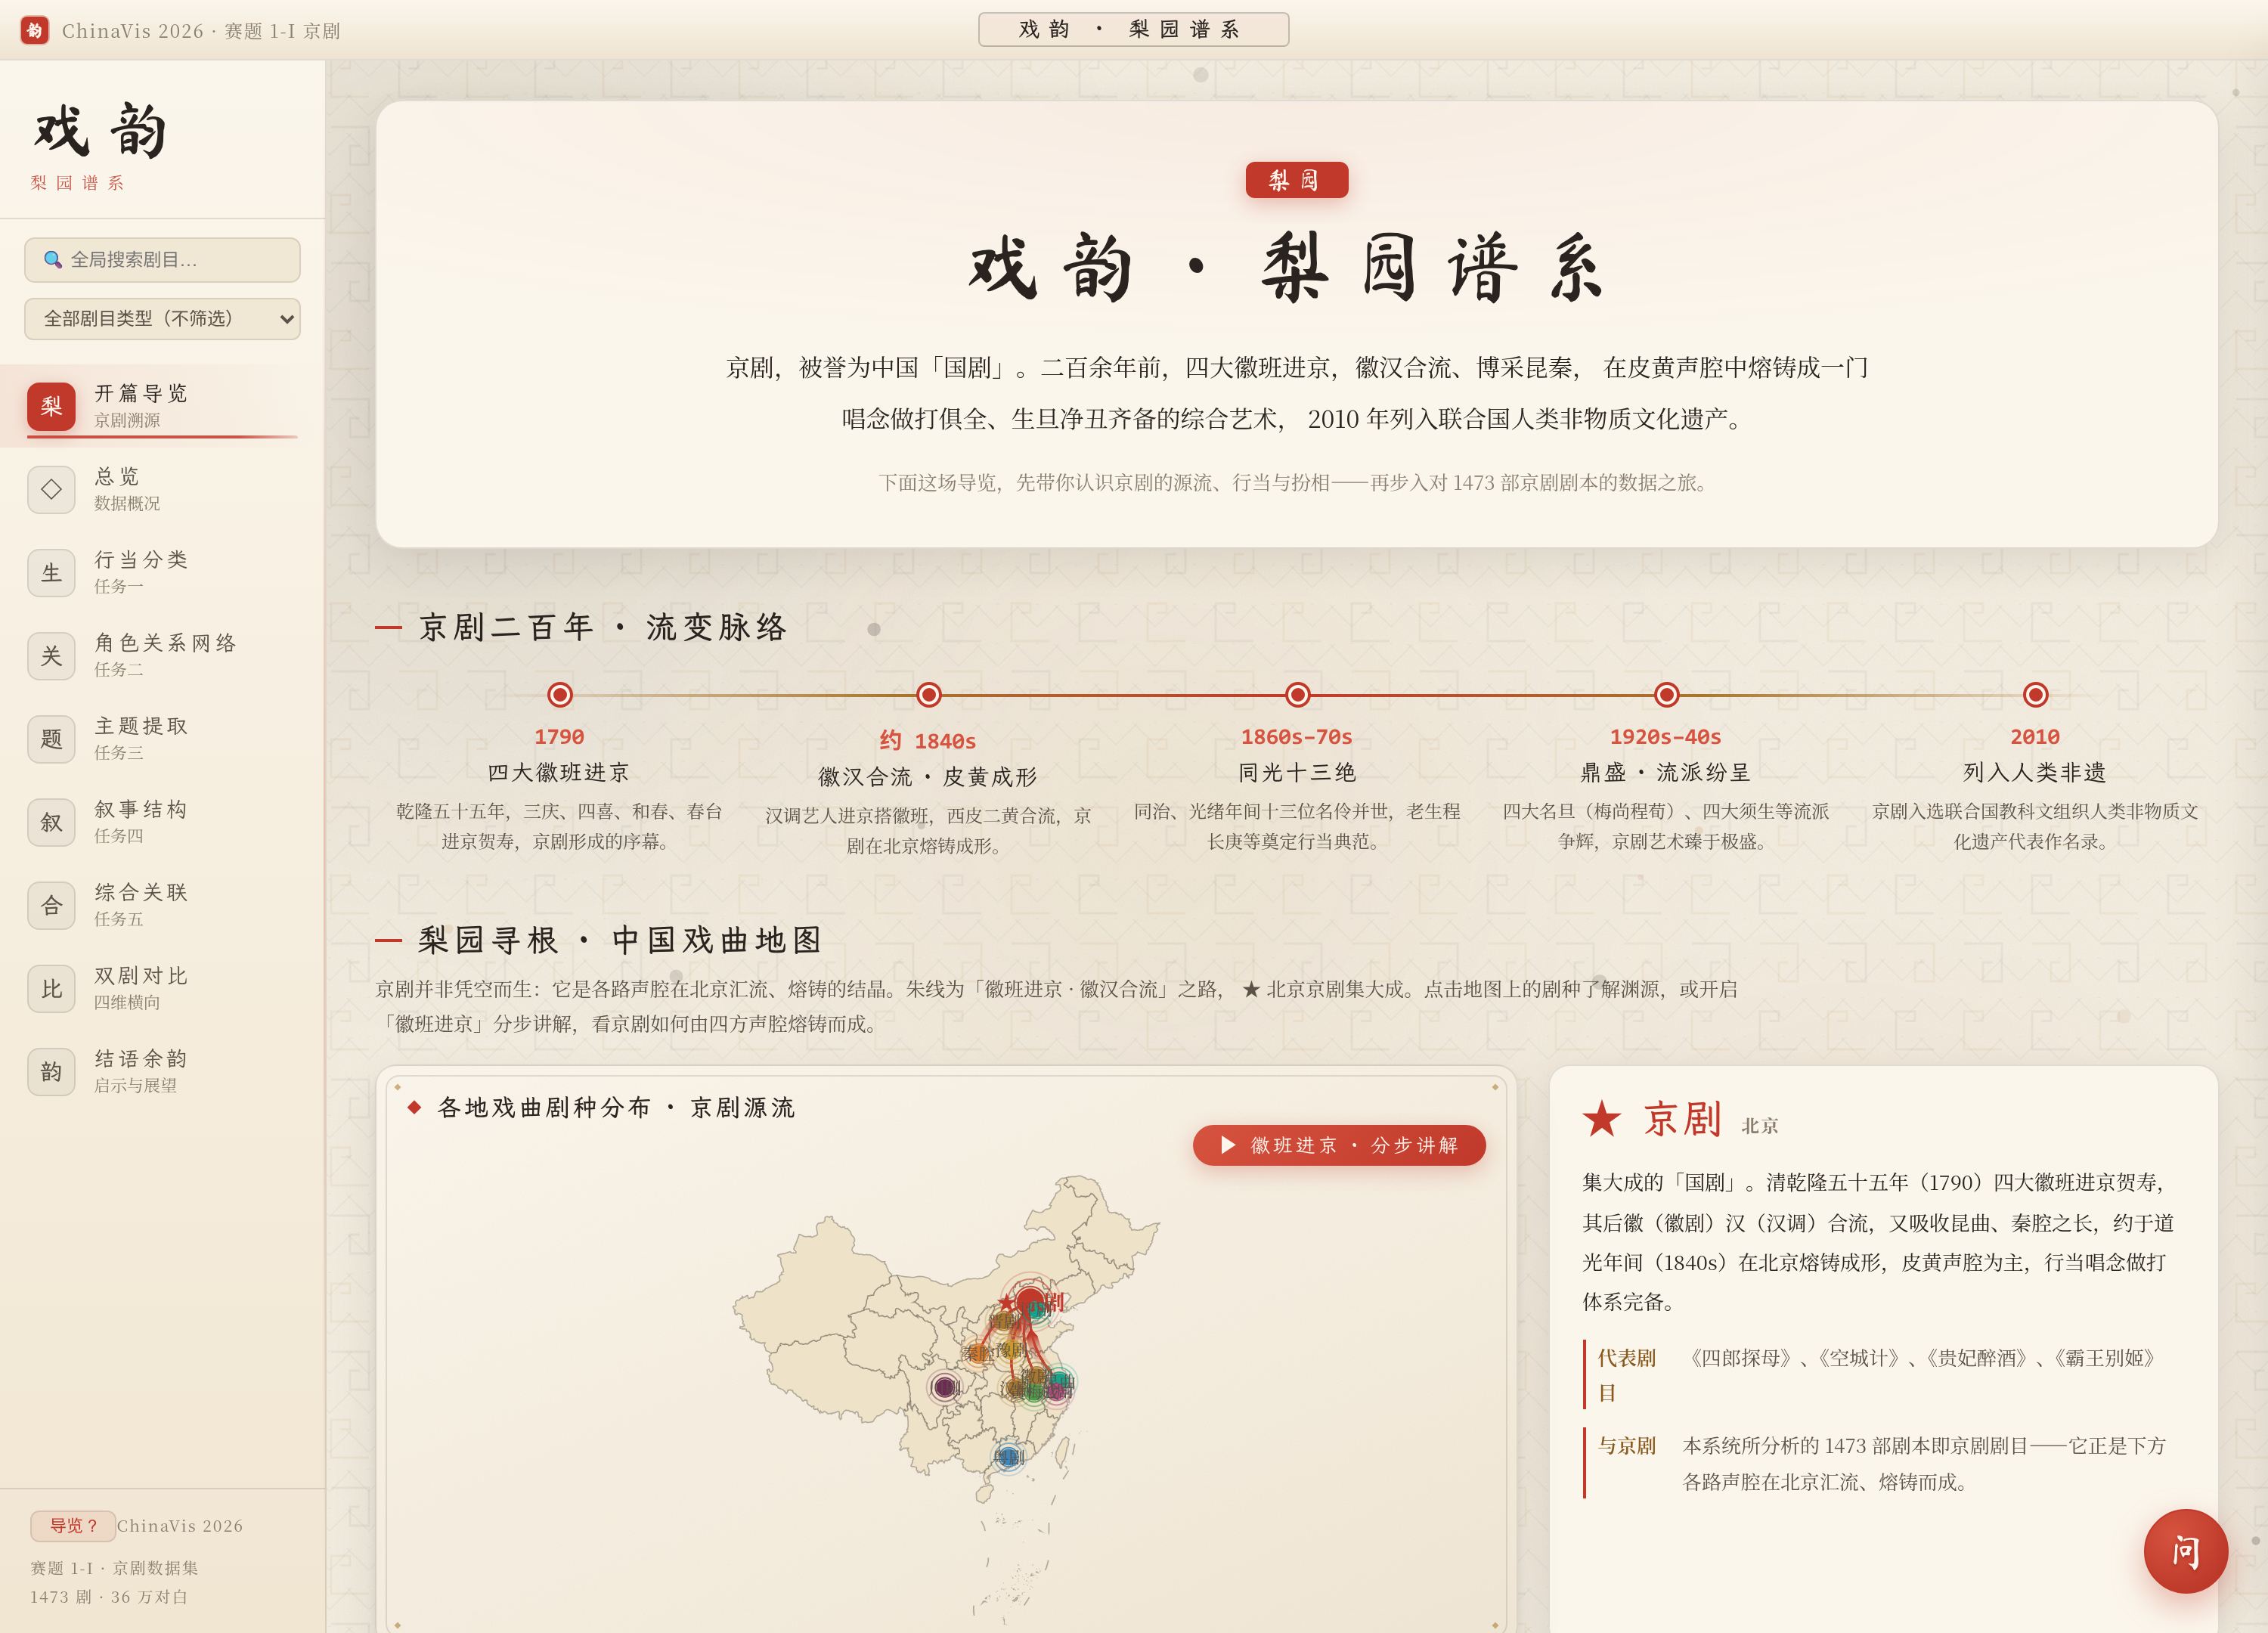
\includegraphics[width=\linewidth]{fig_intro}
  \caption{系统「开篇导览」模块（默认首屏）：以京剧二百年发展时间线、中国戏曲地图（徽班进京 $\cdot$ 徽汉合流的源流叙事）、行当扮相与脸谱象征等为后续数据分析铺陈文化语境，体现「先讲文化、再讲数据」的叙事设计。}
  \label{fig:teaser}
}

\vgtcinsertpkg

\begin{document}

\firstsection{引言}
\maketitle

京剧作为中国戏曲的集大成者，其剧本承载了行当程式、人物关系、题材母题与叙事章法等丰富信息。
ChinaVis 2026 赛题 1-I 提供了一份\emph{跨来源、跨流派}的京剧剧本数据集，要求围绕角色行当分类、
角色关系网络、主题提取、叙事结构与综合关联五个方向开展可视分析。该数据集规模大（1473 部剧本）、
版式半结构化、且缺乏现成标注，使「既要讲清文化、又要讲实数据」成为核心难点。

本文构建的「戏韵 $\cdot$ 梨园谱系」系统针对这一难点做了三方面工作。
\textbf{其一，统一语料底座驱动多任务。} 我们将 38 个来源集合、嵌套压缩的 1473 部 PDF 全部解析为
统一语料（\texttt{corpus.jsonl} 与 \texttt{plays.sqlite}），五项任务共享同一份角色、对白与场次结构，
保证跨任务口径一致、结果可相互印证。
\textbf{其二，叙事化的软件组织。} 系统以「开篇导览（文化语境）$\to$ 总览与任务一至五（数据分析）
$\to$ 结语余韵（升华收束）」的完整叙事弧组织为九个联动模块（见 \autoref{fig:teaser}、\autoref{fig:arch}），
并通过「全局当前剧目」单一真相源实现跨模块四维联动。
\textbf{其三，显式的可信度审计。} 我们不满足于「给出一个数字」，而是对每项分析补充统计学证据：
基线对照与概率校准（任务一）、Erdős–Rényi 零模型 $z$ 值（任务二）、困惑度与一致性驱动选 $K$（任务三）、
silhouette 选簇数与权重敏感性（任务四）、Pearson 相关的 BH-FDR 多重比较校正（任务五）。
这些证据让结论建立在「显著且稳健」的基础上，也诚实地标注了数据局限。

\section{相关工作}
\textbf{戏曲与文学的数字人文。} 以「远读」（distant reading）为代表的计算文学研究，主张用人物网络、
主题分布等量化结构刻画大规模文本~\cite{Moretti:2011:NTP}。剧本天然具备「人物—场次—对白」三元结构，
适合构建角色关系网络并比较不同题材的拓扑特征。本文将这一思路落到京剧语料，并强调与中文戏曲程式
（唱念做打、生旦净丑）相结合的特征工程。
\textbf{文本主题与降维可视化。} 隐含狄利克雷分配（LDA）是主题建模的经典方法~\cite{Blei:2003:LDA}；
为在二维平面观察主题语义关系，我们以主题词分布的 Jensen–Shannon 距离经多维标度（MDS）投影成
「主题分布图」。
\textbf{网络与社群分析。} 我们使用 NetworkX~\cite{Hagberg:2008:NX} 计算规模、密度、Freeman 中心势~\cite{Freeman:1978:CSN}
与模块度~\cite{Newman:2006:MCS}，并以零模型给出显著性参照。
\textbf{机器学习与统计校正。} 行当分类与综合关联分别基于 scikit-learn~\cite{Pedregosa:2011:SL} 的逻辑回归
与相关分析，并以 Benjamini–Hochberg 程序~\cite{Benjamini:1995:CFD} 控制多重比较的假发现率。
与既有工作相比，本文的特色在于\emph{把可信度证据本身做成系统的一部分}，并以叙事弧串联文化语境与数据分析。

\section{数据与预处理}
原始数据为 591\,MB 的压缩包，内含 38 个按来源集合（《戏考》《京剧汇编》《传统剧目汇编》等）
组织的嵌套压缩文件。我们先递归解压（含中文文件名的 GBK 修正），再用 PyMuPDF 抽取文本——
经核验为\emph{可抽取文本而非扫描影像}，故无需 OCR。版式高度统一：每剧含「主要角色」块
（\emph{角色（行当）}）、「情节」摘要、「根据《\dots》整理」出处、以及「【第 $N$ 场】」分场与
「角色（白/念/唱）台词」对白行（全角空格表示续行）。据此我们用规则解析出结构化字段，
最终得到 \textbf{1473} 部剧本（100\% 解析成功）、\textbf{7656} 个「主要角色」行当标注、
\textbf{360{,}223} 条对白，并生成质量报告供抽检。该语料底座以 \texttt{corpus.jsonl}（逐剧 JSON）
与 \texttt{plays.sqlite}（便于检索）两种形态落盘，供后续全部任务复用。

\section{系统设计}
\textbf{总体架构。} 系统采用「数据管线 $\to$ 产物 $\to$ 服务 $\to$ 前端」的分层架构（\autoref{fig:arch}）：
Python 管线（\texttt{pipeline/}）完成解析与五任务离线计算，产物写入 \texttt{data/processed/}；
FastAPI 后端（\texttt{backend/}）以只读方式加载产物并提供 JSON API，其中\emph{建网逻辑前后端共用}
（\texttt{network\_lib.py}），保证「单剧实时建网」与离线统计口径一致；前端（React\,+\,Vite\,+\,ECharts）
为多模块仪表盘，左侧导航在九个模块间切换并支持 \texttt{\#task1} 等深链。系统进一步封装为 Electron
桌面应用（后端随应用自动起停），满足「开发一款专门的软件」的要求。

\begin{figure}[tb]
 \centering
 \begin{tikzpicture}[
   font=\small\sffamily, node distance=3.2mm,
   box/.style={draw, rounded corners=2pt, align=center, inner sep=3pt, minimum height=7mm, fill=black!2},
   arr/.style={-{Latex[length=2mm]}, thick}]
   \node[box, fill=red!6] (raw) {原始数据\\38 来源 $\cdot$ 1473 PDF};
   \node[box, right=of raw] (pipe) {\texttt{pipeline/}\\解析 + 五任务计算};
   \node[box, below=5mm of pipe] (proc) {\texttt{data/processed/}\\语料 + 各任务产物};
   \node[box, left=of proc] (back) {\texttt{backend/}\\FastAPI 只读 API};
   \node[box, below=5mm of back] (front) {\texttt{frontend/} 九模块\\React + ECharts};
   \draw[arr] (raw) -- (pipe);
   \draw[arr] (pipe) -- (proc);
   \draw[arr] (proc) -- (back);
   \draw[arr] (back) -- (front);
   \node[draw, dashed, rounded corners, fit=(back)(front), inner sep=4pt, label={[font=\scriptsize\sffamily]below:Electron 桌面封装}] {};
   \node[right=1mm of pipe, font=\scriptsize, text width=2.2cm, align=left] {\texttt{network\_lib.py}\\前后端共用建网};
 \end{tikzpicture}
 \caption{系统分层架构：离线管线产出统一产物，后端只读服务，前端九模块仪表盘；建网逻辑前后端共用以保证口径一致。}
 \label{fig:arch}
\end{figure}

\textbf{叙事弧与联动。} 九个模块按叙事弧组织：开篇导览（\autoref{fig:teaser}）以时间线、戏曲地图与行当扮相
铺陈文化语境；总览（\autoref{fig:overview}）给出数据概况；任务一至五为分析主体；双剧对比提供四维横向
比较；结语余韵实时取真实指标综述统一故事。系统以\textbf{全局「当前剧目」}为单一真相源（localStorage 持久）：
在侧栏检索任一剧目后，五个任务模块自动联动展示该剧的行当、网络、主题、叙事与四维档案；
另设\textbf{跨图剧目类型筛选}，五任务全库视图统一响应。系统还内置「数据接地」的 AI 助手：
将已算出的全库指标与当前剧目画像拼为上下文，仅依据真实数据作答。

\begin{figure*}[tb]
 \centering
 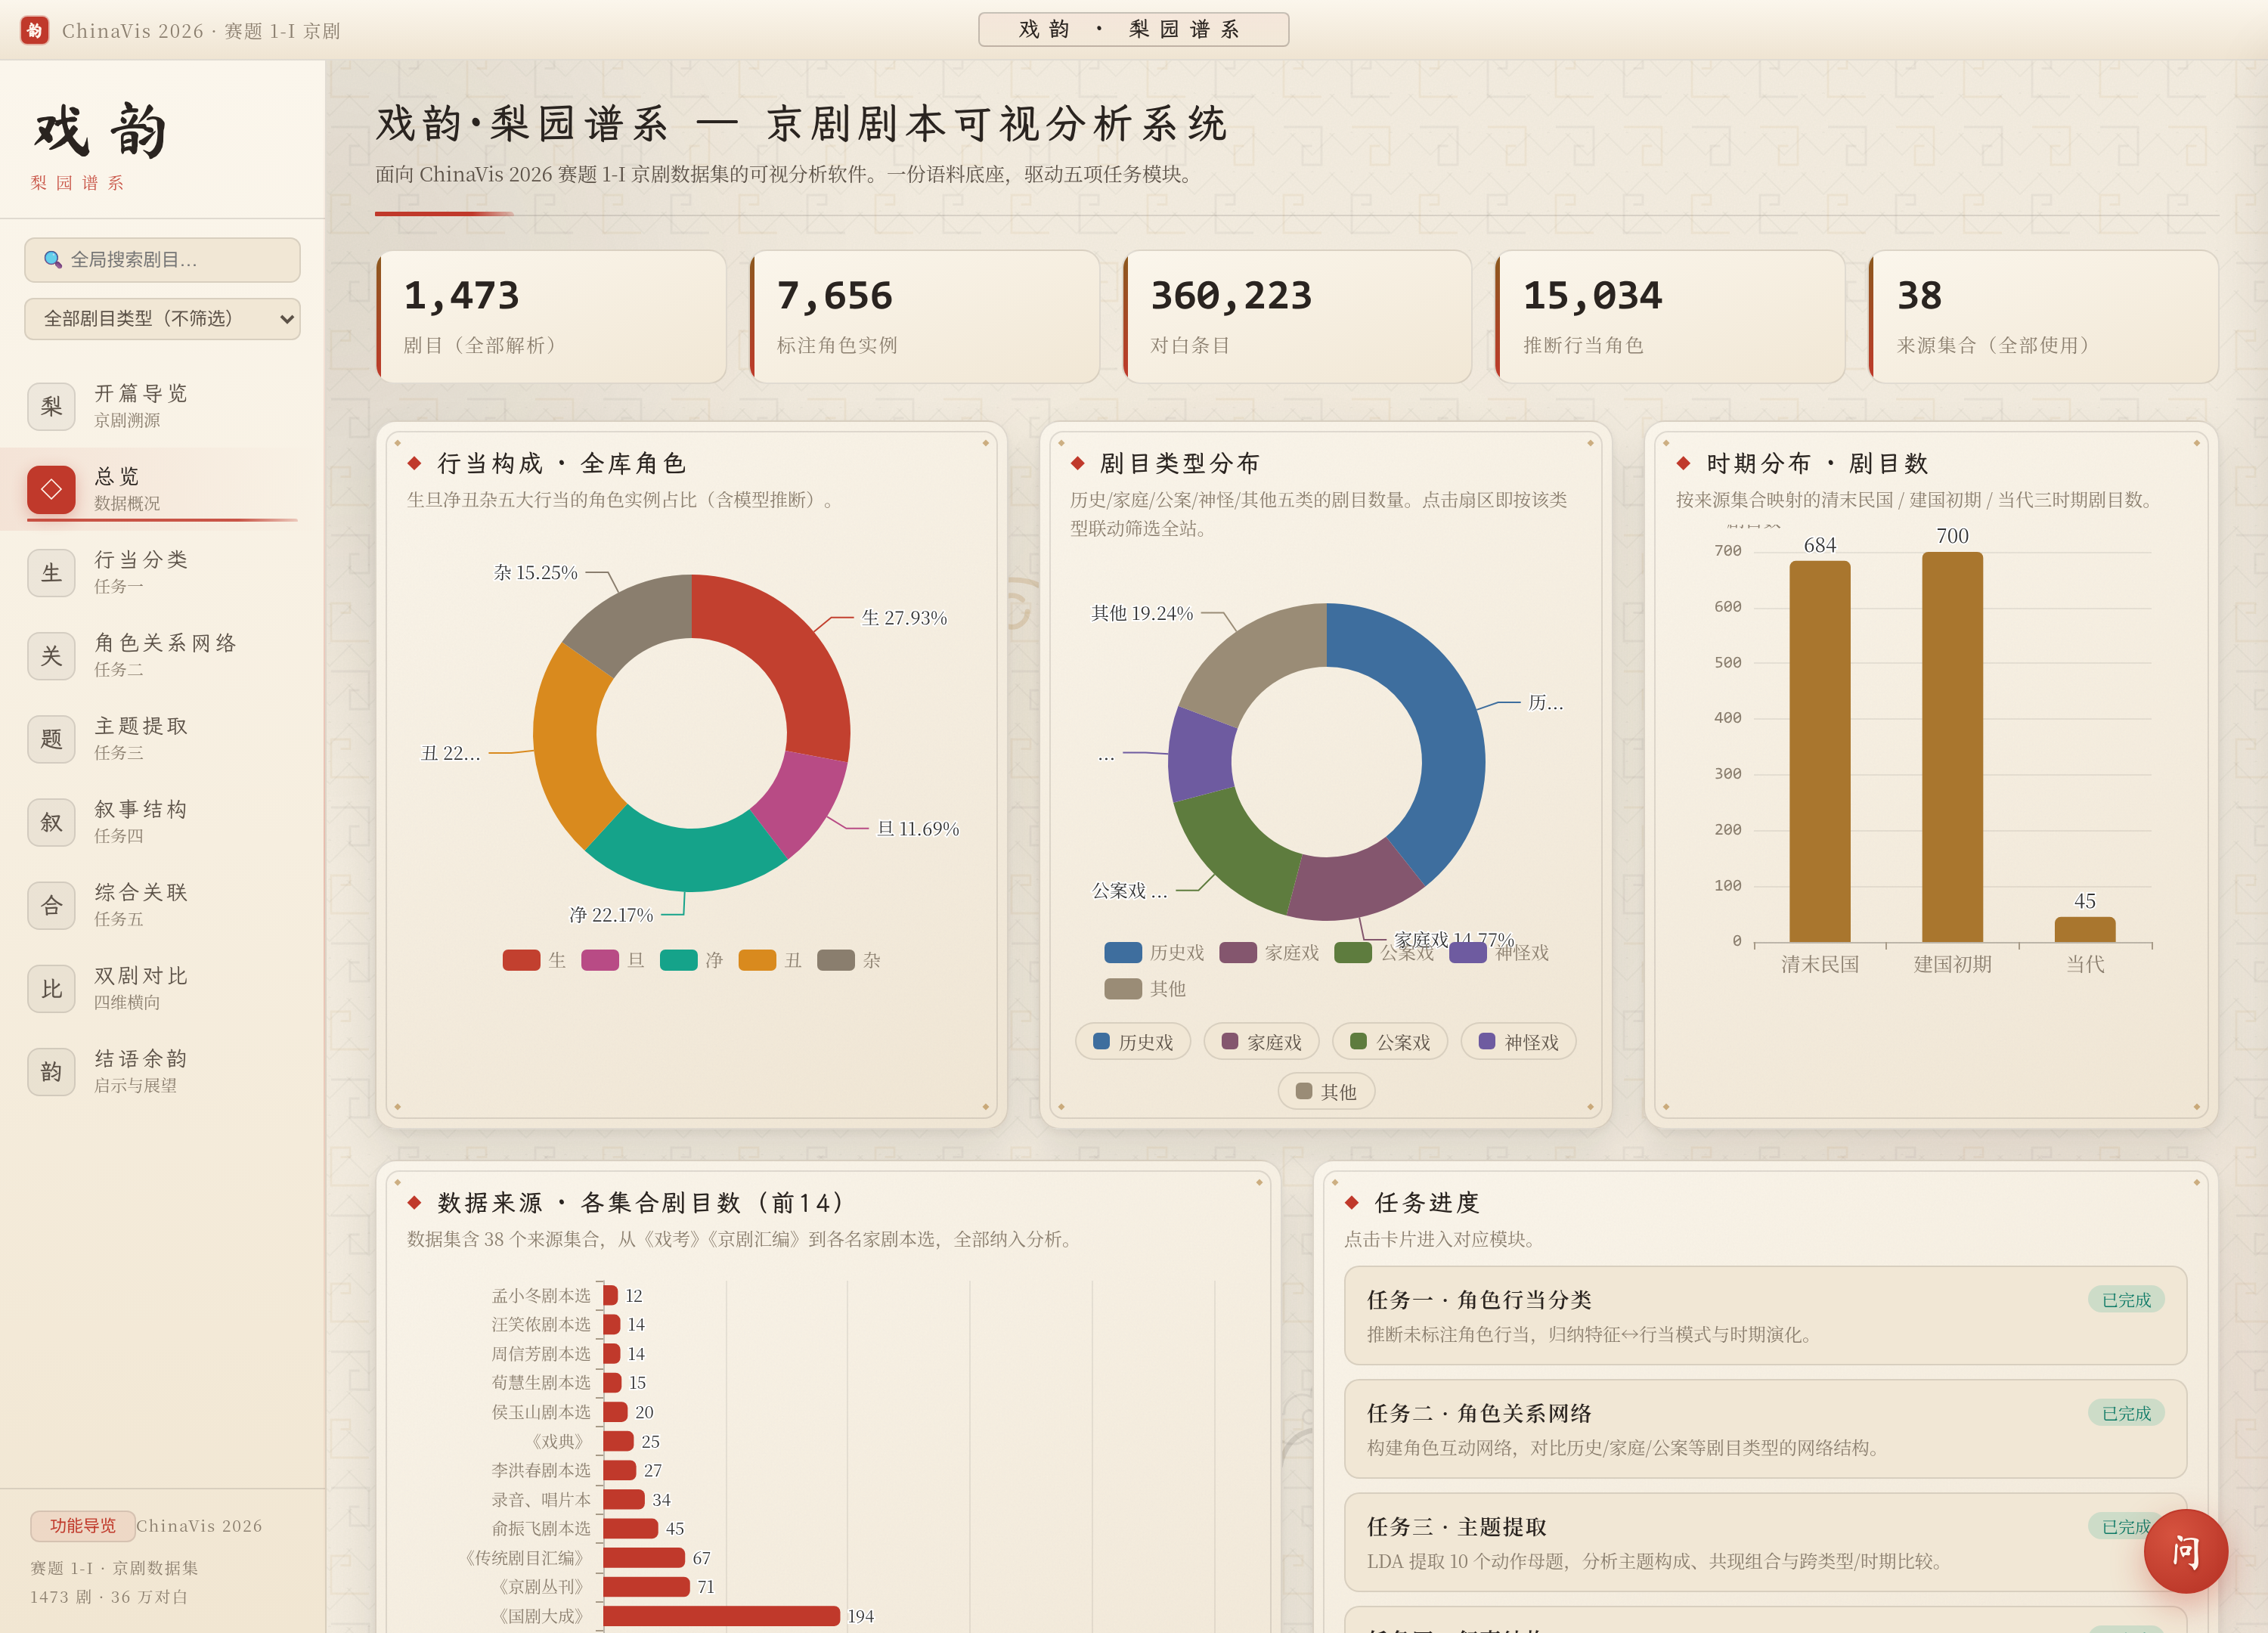
\includegraphics[width=0.8\linewidth]{fig0_overview}
 \caption{总览模块：数据规模 KPI（动态计数）、五任务一览与全库概况，作为「开篇导览」到逐任务深入的过渡。}
 \label{fig:overview}
\end{figure*}

\section{任务分析与发现}
本节逐一介绍五项任务的方法、关键视图与发现，并特别说明每项分析的可信度证据。各任务关键发现汇总见
\autoref{tab:summary}。

\subsection{任务一：角色行当分类与时期演化}
\textbf{方法。} 从「主要角色」块解析出 7656 个行当标注，其中 \textbf{7428} 个能与对白说话人精确匹配、
作为实例级训练样本；特征涵盖唱/念/白占比、台词量、出场场次、共现度、性别/年龄身份关键词与台词 TF-IDF，
以逻辑回归 Pipeline 训练（末行并入生行，杂行作群演辅助类）。
\textbf{可信度。} 实例级 5 折 \textbf{macro-F1 $=0.704$}、按剧目分组验证 $0.696$、官方四类（生/旦/净/丑）$0.753$。
为说明「这个分数是否够用」，我们给出\textbf{基线对照}：多数类 DummyClassifier 仅 $0.118$、随机森林 $0.552$，
逻辑回归显著更优；并做\textbf{概率校准}（多类 Brier $=0.349$ 与可靠性曲线，见 \autoref{fig:task1} 右上），
据此对 15{,}034 个未标注出场角色的推断按高/中/低置信度（$5670/4129/5235$）分级，低置信样本在界面标为「待核」。
\textbf{时期演化。} 以来源集合映射时期（清末民国/建国初期/当代），净行占比持续下降（$0.224\to0.212\to0.163$）。
卡方检验显示时期与行当分布的关联\emph{统计显著}（$\chi^2=39.2$, $p=6.5\times10^{-7}$），但 Cramér's V $=0.052$ 表明
\emph{效应极弱}——我们据此给出诚实结论：行当结构总体稳定，变化虽显著但量级很小。
\textbf{细分行当。} 分层分类下，生行细分（老生/小生/武生/红生/娃娃生）5 折 macro-F1 达 $0.733$、旦行 $0.560$；
净/丑因标注稀疏且缺铜锤/架子等核心区分，\emph{仅展示已标注细分、不作推断}（诚实声明数据局限）。
\textbf{误判结构（零重训）。} 将交叉验证混淆矩阵按行归一为召回视角（\autoref{fig:task1}），最大误判集中在
\textbf{生$\leftrightarrow$净}（生$\to$净 411 例、净$\to$生 374 例；二者同以念白为主、舞台气质相近），杂行召回最低；
误判结构与表演型重叠一致，说明 macro-F1 的上限源自数据本身的行当边界模糊而非模型缺陷，并为人工复核给出优先级。

\begin{figure*}[tb]
 \centering
 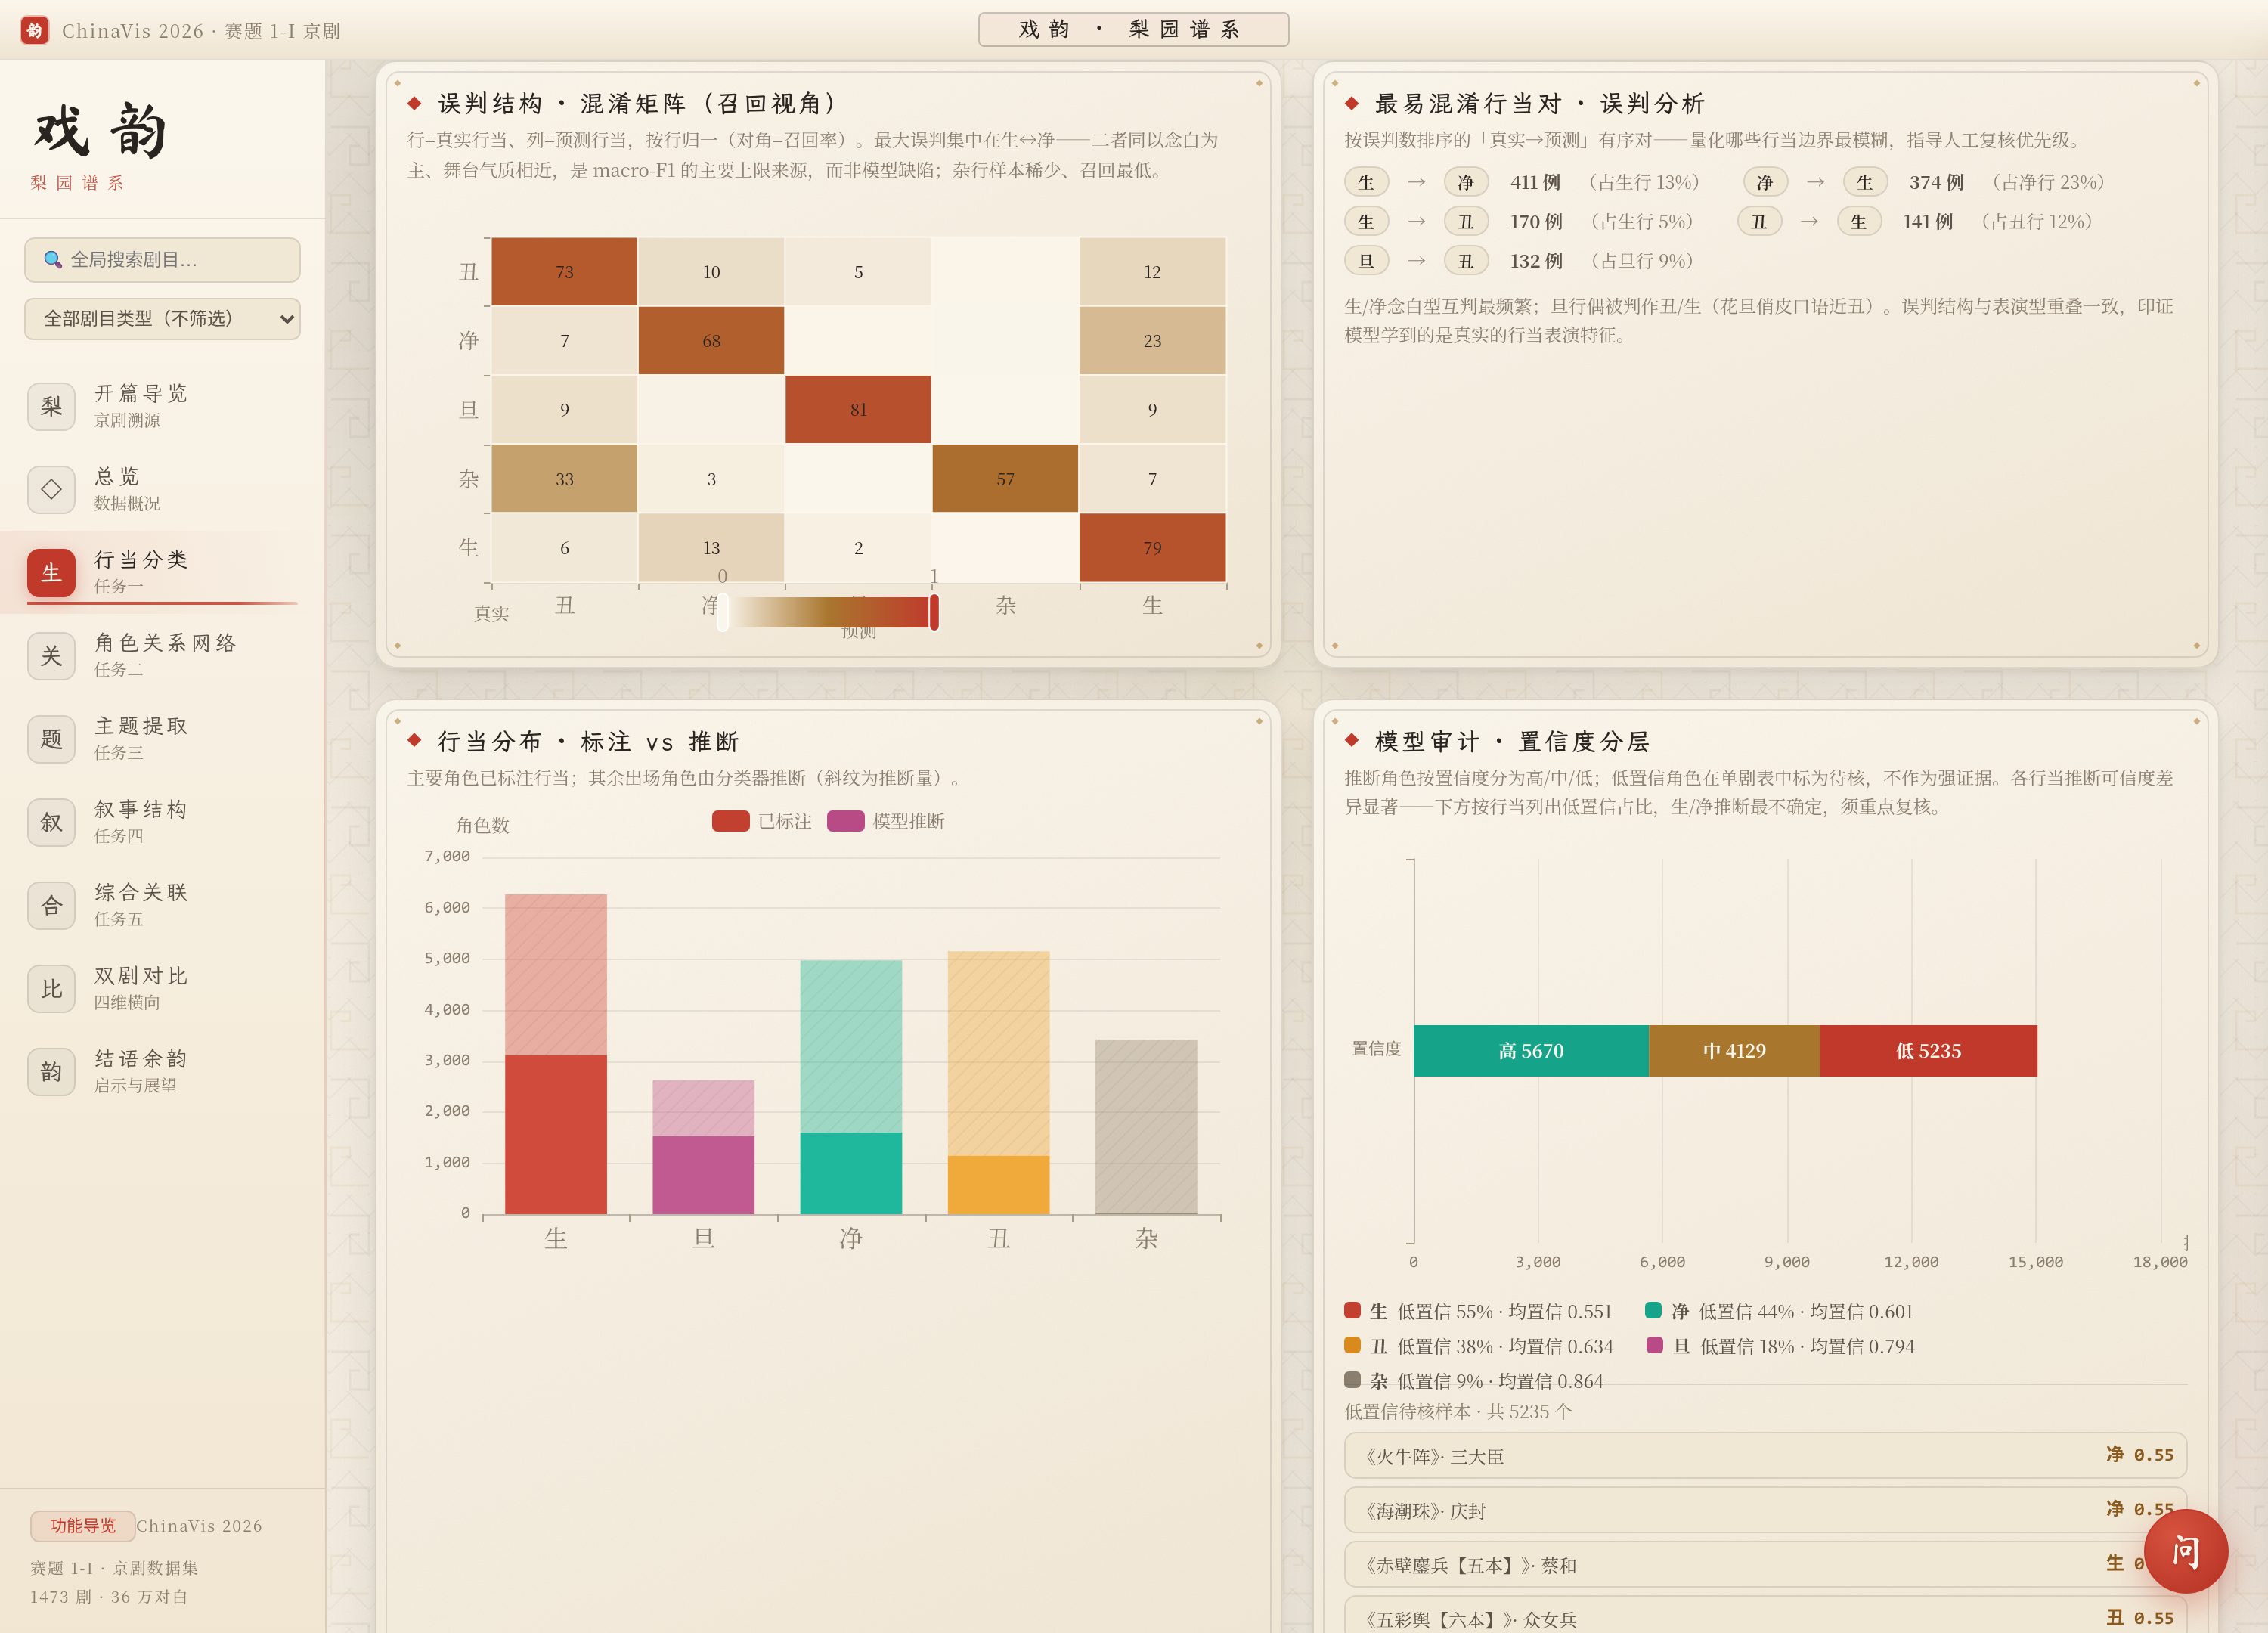
\includegraphics[width=0.8\linewidth]{fig1_roles}
 \caption{任务一界面：误判结构混淆矩阵（召回视角）与最易混淆行当对（生$\leftrightarrow$净），并置基线对照、置信度可靠性曲线、行当分布与推断置信分层——可信度证据与分类结果并陈。}
 \label{fig:task1}
\end{figure*}

\subsection{任务二：角色关系网络结构特征}
\textbf{方法。} 以「同场共现 $+$ 对话邻接」定义角色互动，对 1462 部剧用 NetworkX 建网，计算规模、密度、
平均度、Freeman 中心势、聚类系数与模块度；并按情节/标题关键词将剧目分为历史戏(580)、公案戏(241)、
家庭戏(212)、神怪戏(143)与其他(286)。
\textbf{发现（\autoref{fig:task2}）。} 公案戏网络规模最大（均 15.4 角色/68.6 关系）、中心势高（$0.30$，并列最高档），
呈以清官/判官为核心的星型结构；历史戏模块度最高（$0.21$），网络分裂为敌我/朝野多社群；
家庭戏规模最小但密度最高（$0.70$），人物少而互动紧密。
\textbf{可信度。} 为排除「大网络自然模块度更高」的混淆，我们对每剧生成 20 个同规模 Erdős–Rényi 零模型，
计算指标的 $z$ 值。历史戏的模块度 $z=3.23$ 为各类型最高，证明其社群结构\emph{显著强于随机预期}，而非规模副产物。
进一步对各类型指标做\textbf{两两 Mann–Whitney U 检验}（BH-FDR）：历史戏模块度显著高于家庭戏，但与公案、神怪戏
差异\emph{未达显著}（故「模块度并列最高档」更准确）；公案戏规模显著大于其余类型。
\textbf{结构角色与阵营同质度。} 逐节点计算度/介数中心性并按行当聚合——\textbf{生行连接最广、介数最高、约 51\%
剧目占据「桥接主座」}（剧情组织者），净次之、杂行最外围；各类型行当同配系数 role assortativity \textbf{均为负}
（全库 $-0.16$）：人物网络按行当「互补异配」（生旦净丑交错搭戏），社群对应「敌我阵营」而非「同行当抱团」。
\textbf{时期演化。} 网络规模随时代\emph{显著增大}（Kruskal–Wallis 显著，均 $10.8\to15.4\to18.3$ 角色），
人物体系趋于庞大复杂，模块度/中心势在建国初期达峰（\autoref{fig:task2}）。

\begin{figure*}[tb]
 \centering
 \includegraphics[width=0.8\linewidth]{fig2_network}
 \caption{任务二界面：结构角色散点（度$\times$介数中心性，生行居桥接核心）与各类型行当同配系数（均为负$=$互补异配）、类型差异显著性矩阵（▲显著更高/▼更低/·不显著）、网络结构时期演化曲线（规模随时代增大）。}
 \label{fig:task2}
\end{figure*}

\subsection{任务三：核心主题提取与组合模式}
\textbf{方法与净化。} 以各剧「情节」摘要（覆盖 99.5\%）为语料，jieba 词性标注仅保留名/动/形内容词。
为防主题退化为人名/道具，做两层实体净化：① 用数据自身角色名构建黑名单并补「黄三泰$\to$三泰」等裸名变体；
② 按\emph{故事}归并多卷剧（头本/二本/【三本】\dots）后计文档频率，剔除只在极少数故事出现的剧目专属名/道具。
\textbf{数据驱动选 $K$。} 对 $K=5\dots15$ 扫描 u\_mass 一致性，在 $K=10$ 取得最优后回落，按「一致性退化前
最细划分」取 $\mathbf{K=10}$（而非硬选粒度）。
\textbf{发现（\autoref{fig:task3}）。} 净化后 10 个主题对应清晰的动作母题——征战、忠义复仇、婚姻家庭、断狱等；
主题共现显示「征战$\times$忠义复仇」「婚姻$\times$家庭」为高频稳定组合；KMeans 得 6 个原型组合，最大原型
（约 500 部）以「征战$+$复仇」为主干。以主题词分布的 JS 距离经 MDS 投影的「主题分布图」可见母题语义聚簇。
\textbf{时期迁移。} 逐主题对三时期每剧权重做 Kruskal–Wallis 检验（BH-FDR），10 母题占比变化全部显著：
征战类母题随时代\emph{下降}（攻打/出战 $-6.3$pt、进京/镇守 $-4.2$pt），家庭伦理类\emph{上升}（妻子/投江 $+7.3$pt、
母女/父子 $+7.6$pt）——题材由「武戏征战」向「家庭伦理」迁移（\autoref{fig:task3}）。
\textbf{稳健性对照。} 以主题-词分布的最优匹配余弦衡量复现度，LDA 主题与完全不同的 NMF 方法平均一致 $0.46$、
多 seed LDA 平均一致 $0.54$，复仇/家庭杀戮/救援等核心母题高度复现（余弦 $0.6$–$0.9$），印证「10 母题」非单次
随机产物（部分征战母题细分边界存在方法依赖性，诚实声明）。

\begin{figure*}[tb]
 \centering
 \includegraphics[width=0.8\linewidth]{fig3_topics}
 \caption{任务三界面：主题随时代变迁折线（红升/青降，征战降、家庭伦理升）、主题稳健性 NMF/多 seed 对照（核心母题高复现），核心主题占比与主题分布图（JS 距离 $+$ MDS）。}
 \label{fig:task3}
\end{figure*}

\subsection{任务四：叙事结构与典型叙事模式}
\textbf{方法。} 以表演形式标记合成逐场「戏剧强度」曲线：唱腔(文)$=$该场唱占比、武打(武)$=$舞台提示中
做打动作标记密度（起霸/开打/趟马/圆场\dots）、冲突$=$发言人切换率$\times$同场人数；综合强度
$=0.4\cdot\text{文}+0.4\cdot\text{武}+0.2\cdot\text{冲突}$，各按全剧归一。据峰值识别开端/发展/高潮/结局，
并将曲线重采样为 16 点后对 965 部（$\ge4$ 场）剧目作 KMeans 聚类。
\textbf{可信度。} 簇数由 silhouette（$K=2\dots8$，曲线平缓 $0.12$–$0.14$）权衡选 $K=5$——以极小代价换取
5 种可辨弧形；并做\textbf{权重敏感性}：6 组权重全走同一管线与采用权重比 ARI，$\pm0.1$ 文武微调仍维持
$0.55$–$0.60$（中等稳健），文武平衡最敏感。
\textbf{发现（\autoref{fig:task4}）。} 得 5 种名称互异的典型弧线：平稳铺陈式(288)、结尾陡升式(202)、
后段高潮式(181)、前段先声夺人式(151)、中段经典弧线式(143)，各可叠加簇内 p25–p75 离散度带。
全库高潮位置右偏，印证「层层铺垫、后段收束」的戏曲惯例；历史戏做打最多（均 5.0）、节奏外放，
家庭/公案戏更依赖唱念抒情。类型间\textbf{两两 Mann–Whitney U 检验}（BH-FDR）显示：历史戏做打量显著高于家庭戏
与神怪戏，但与公案戏差异\emph{未达显著}——「历史戏做打最多」成立但需限定比较对象（\autoref{fig:task4}）。

\begin{figure*}[tb]
 \centering
 \includegraphics[width=0.8\linewidth]{fig4_narrative}
 \caption{任务四界面：类型节奏差异显著性矩阵（做打量/高潮位置/唱腔占比，▲显著更高/▼更低/·不显著）、5 种典型叙事弧线原型（可叠加 p25–p75 带）与高潮位置分布。}
 \label{fig:task4}
\end{figure*}

\subsection{任务五：综合关联与协同演化}
\textbf{方法。} 打通任务二（关系）、三（主题）、四（叙事）与行当构成，构建每剧四维联合特征，计算跨维度
Pearson 相关矩阵、「类型$\to$主题$\to$叙事」协同链路（Sankey），并在联合空间 KMeans 聚出综合原型。
\textbf{可信度。} 对 96 对相关做 Benjamini–Hochberg FDR 校正，其中 \textbf{37} 对在 $p_{\text{adj}}<0.05$ 下显著，
头条相关全部显著；界面中非显著格降透明度、关联发现卡片标注 $p$ 值与 $R^2$（\autoref{fig:task5}）。
\textbf{发现。} 网络规模$\leftrightarrow$武打量 $r=+0.58$、模块度$\leftrightarrow$武打量 $+0.45$、
模块度$\leftrightarrow$净占比 $+0.35$、模块度$\leftrightarrow$旦占比 $-0.32$——大而分阵营的网络多承载征战题材、
武打高潮、由净行主导；旦行为主的戏则网络更紧凑单核。Sankey 显示「历史戏$\to$征战$\to$结尾渐强」与
「家庭戏$\to$婚姻家庭$\to$平稳/前段叙事」等稳定链路；联合聚类得 6 类综合原型。
\textbf{偏相关控混淆（甄别真假协同）。} 大戏「既人多分阵营、又做打多」，原始相关可能由共同「剧目体量」驱动。
补「控制网络规模/场次后的偏相关」——37 显著项中 \textbf{26 项控体量后仍稳健}：行当协同为真（模块度$\leftrightarrow$净占比
$+0.35\to+0.21$、$\leftrightarrow$旦占比 $-0.32\to-0.22$），而\textbf{「模块度/密度$\leftrightarrow$武打」实为体量假象}
（$+0.45\to+0.02$、$-0.51\to-0.06$）。\textbf{轻量预测验证}进一步把「协同」升级为「可由 A 预测 B」：仅用非叙事
维度交叉验证预测叙事弧型，macro-F1 $=0.226$ 约为多数类基线（$0.092$）的 $2.5$ 倍——四维确有可预测耦合，
但绝对精度不高、叙事保有自身变异，与偏相关结论相互印证。

\begin{figure*}[tb]
 \centering
 \includegraphics[width=0.8\linewidth]{fig5_synthesis}
 \caption{任务五界面：跨维度相关热力图，带 $p$ 值/$R^2$/偏相关（控体量 $r$）的关联发现卡（26/37 项控体量后稳健），轻量预测验证（macro-F1 $=0.226$ vs 基线 $0.092$）。}
 \label{fig:task5}
\end{figure*}

\begin{table}[tb]
 \caption{五项任务的方法、可信度证据与关键发现汇总。}
 \label{tab:summary}
 \scriptsize
 \centering
 \begin{tabular}{@{}p{0.10\columnwidth}p{0.34\columnwidth}p{0.42\columnwidth}@{}}
  \toprule
  任务 & 可信度证据 & 关键发现 \\
  \midrule
  一 行当 & 基线对照$+$校准$+$$\chi^2$/V$+$混淆矩阵 & macro-F1 0.704；最大误判生$\leftrightarrow$净；净行随时期降但效应极弱 \\
  二 网络 & ER 零模型 $z$$+$两两 MWU$+$时期 KW & 公案重核心、历史重阵营；生行居桥接核心、行当互补异配；规模随时代增大 \\
  三 主题 & u\_mass 选 $K{=}10$$+$NMF/多 seed 稳健 & 10 母题，征战降/家庭伦理升；核心母题跨方法高复现 \\
  四 叙事 & silhouette$+$权重敏感性$+$两两 MWU & 5 种互异弧线；历史戏做打显著高于家庭/神怪戏 \\
  五 综合 & BH-FDR$+$偏相关控混淆$+$预测验证 & 规模$\leftrightarrow$武打 $r{=}{+}0.58$；行当协同稳健、武打协同实为体量假象 \\
  \bottomrule
 \end{tabular}
\end{table}

\section{讨论与局限}
本系统在「讲清文化」与「讲实数据」之间取得了平衡，但仍有若干诚实需声明的局限。
\textbf{时期为来源代理。} 我们以来源集合近似剧本年代，并非精确创作年份，故时期演化结论应作趋势性解读。
\textbf{标注稀疏。} 净/丑行当细分标注稀少且不含铜锤/架子等核心区分，因此细分推断仅对生/旦建模。
\textbf{词袋局限。} 任务三基于 LDA 词袋，主题为「动作母题」而非情感/价值主题，且依赖分词与实体净化质量。
\textbf{强度为代理量。} 任务四的「戏剧强度」由表演形式标记合成，是叙事节奏的可解释代理而非观众感知的真实强度。
尽管如此，我们对每一结论都附了统计显著性与稳健性证据，并在系统「结语余韵」中明确这些边界，
力求结论\emph{不被过度解读}。

\section{结论}
我们构建并实现了「戏韵 $\cdot$ 梨园谱系」——一个以统一语料底座驱动五项任务、以叙事弧组织为九个联动模块的
京剧剧本可视分析系统。系统不仅给出行当分类、关系网络、主题母题、叙事弧线与综合关联的可视化结果，
更将基线对照、概率校准、零模型、选 $K$、权重敏感性与多重比较校正等\emph{可信度证据本身做成系统的一部分}。
分析表明，京剧的人物关系拓扑、主题母题与叙事节奏并非彼此独立，而是存在典型关联模式与协同演化规律
（如网络规模与武打量 $r{=}{+}0.58$ 的强协同），题材决定人物关系拓扑与行当配置，进而塑造叙事节奏；
可交互系统支持从任一维度反查另两维，实现统计特征与剧本结构的双向印证。

\acknowledgments{
感谢 ChinaVis 2026 组委会提供京剧数据集。本作品为「数据可视化 2026」课程考核作品。}

\bibliographystyle{abbrv-doi}
\bibliography{template}
\end{document}
